\documentclass{article}

\usepackage{graphicx}
\usepackage{tikz}
\usepackage{tikzsymbols}
\usetikzlibrary{calc,patterns,shapes.geometric}
\pagestyle{empty}
\usepackage[margin=0pt]{geometry}
\geometry{papersize={14in,12in}}

\def\centerarc[#1](#2)(#3:#4:#5){\draw[#1] ($(#2)+({#5*cos(#3)},{#5*sin(#3)})$) arc (#3:#4:#5);}

\begin{document}
	\begin{figure}
		\centering
		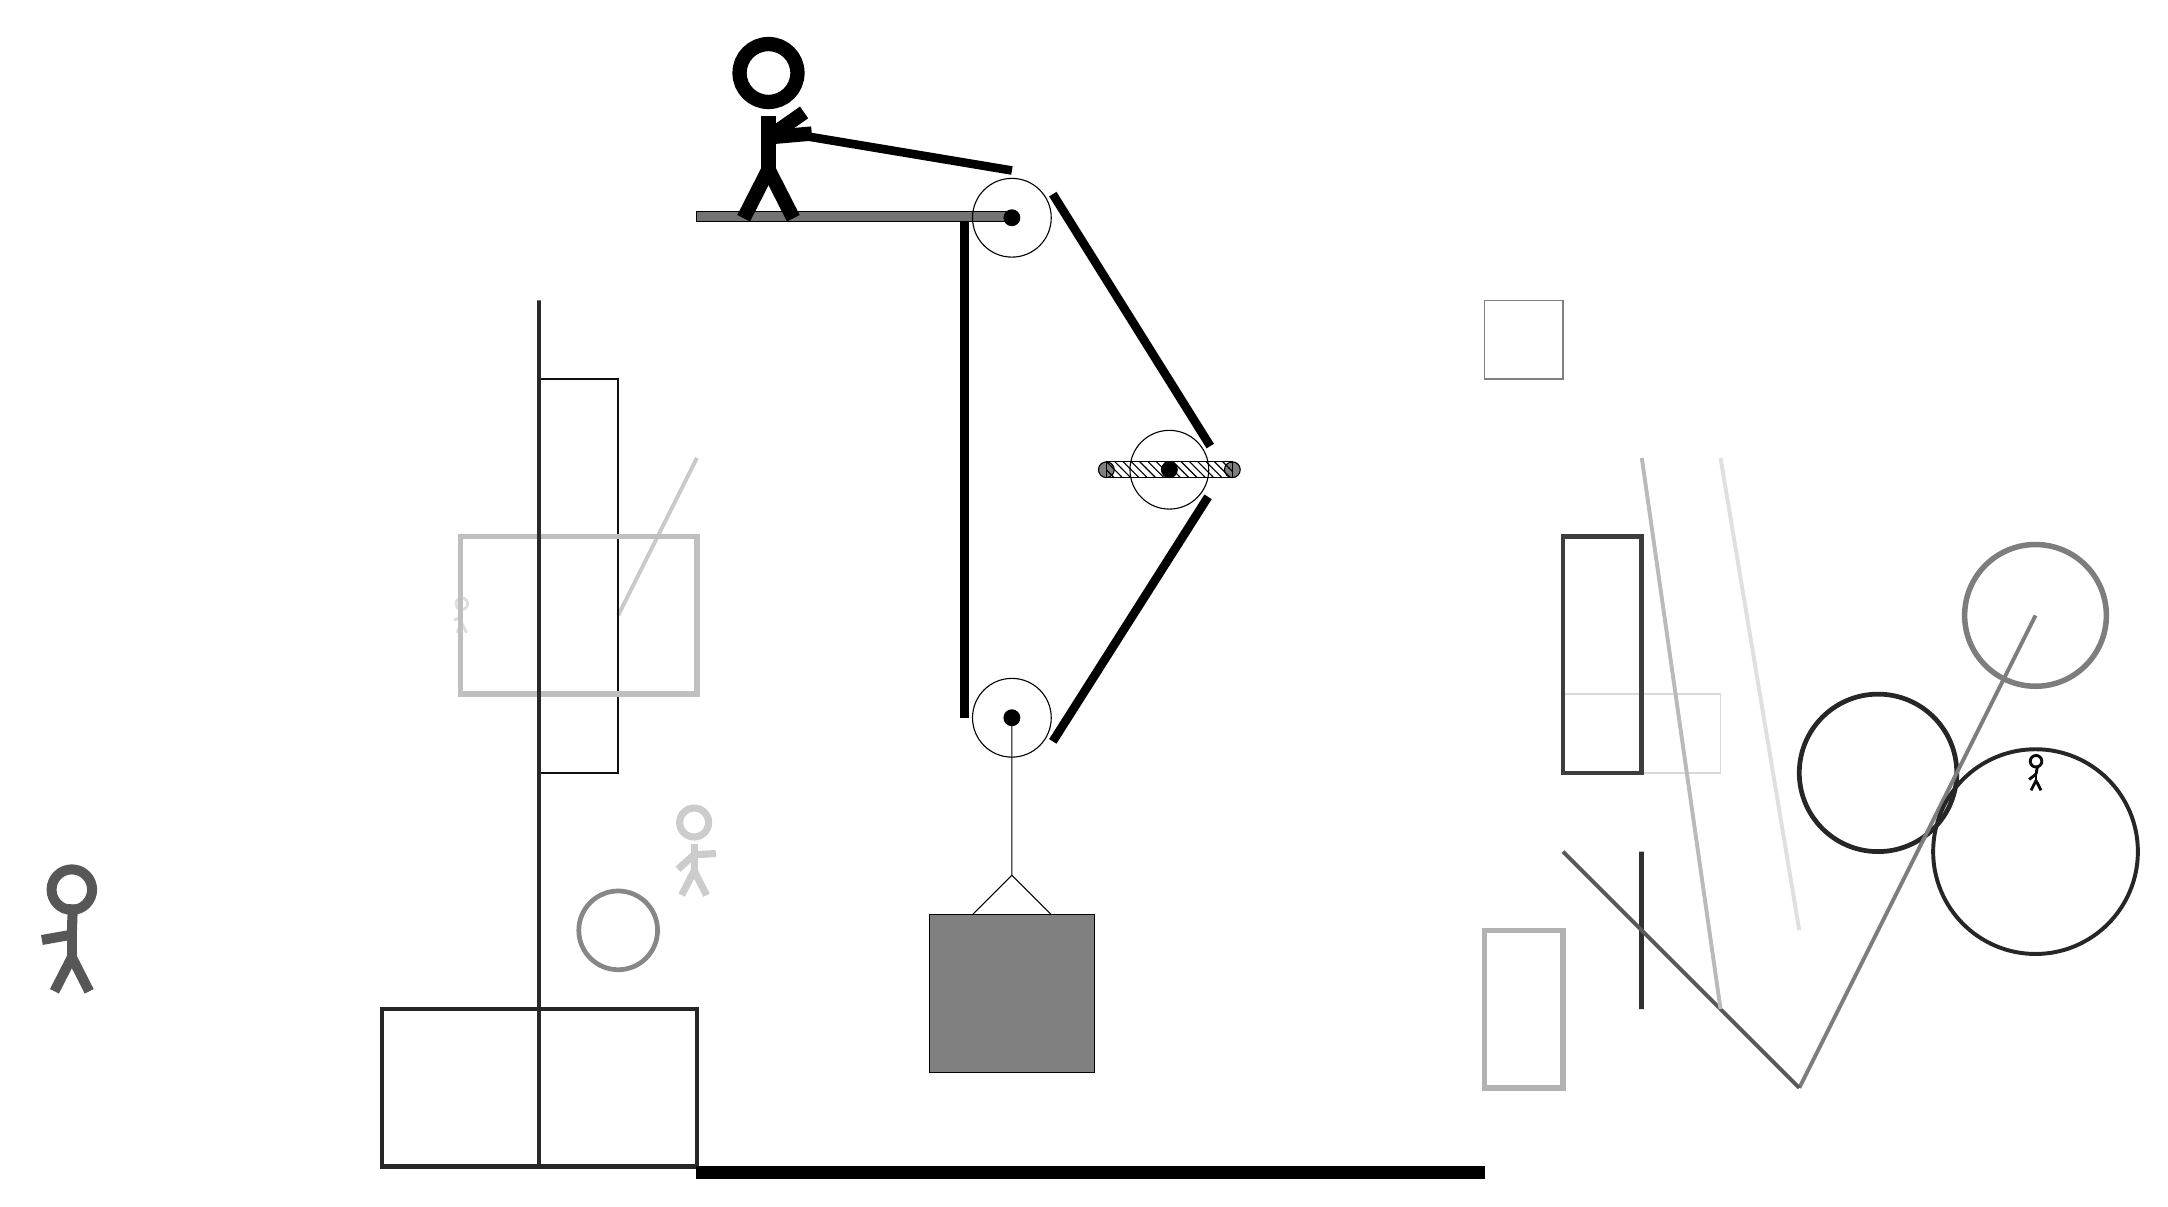
\begin{tikzpicture}
			%%%%% START %%%%%
			
			\draw[fill=black!55] (-2, 9) rectangle (2, 9.125);
			
			\draw (2, 2.7) circle (0.5);
			\draw[fill=black] (2, 2.7) circle (0.1);
			
			\draw [line width=0.7mm, color=black!51](15, 4) circle (0.9);
			
			\draw[line width=0.2mm, color=black!50] (9, 7) rectangle (8, 8);
			\draw [line width=0.6mm, color=black!85](13, 2) circle (1.0);
			\draw[line width=0.5mm, color=black!21](-2, 6) -- (-3, 4);
			\draw[line width=0.2mm, color=black!15] (9, 3) rectangle (11, 2);
			\node[line width=0.6mm, color=black!20] at (-2, 1) {\Strichmaxerl[5][42][3]};
			\draw[line width=0.5mm, color=black!12](11, 6) -- (12, 0);
			
			\node[line width=0.7mm, color=black!96] at (15, 2) {\Strichmaxerl[2][38][79]};
			\node[line width=0.6mm, color=black!13] at (-5, 4) {\Strichmaxerl[2][25][90]};
			\draw[line width=0.5mm, color=black!51](12, -2) -- (15, 4);
			\draw[line width=0.3mm, color=black!94] (-3, 7) rectangle (-4, 2);
			
			\draw [line width=0.6mm, color=black!47](-3, 0) circle (0.5);
			\draw[line width=0.6mm, color=black!76] (9, 2) rectangle (10, 5);
			
			\node[line width=0.5mm, color=black!66] at (-10, 0) {\Strichmaxerl[7][10][88]};
			\draw[line width=0.7mm, color=black!25] (-2, 3) rectangle (-5, 5);
			\draw[line width=0.7mm, color=black!30] (8, -2) rectangle (9, 0);
			\draw[line width=0.6mm, color=black!81] (10, -1) rectangle (10, 1);
			\draw[line width=0.5mm, color=black!65](9, 1) -- (12, -2);
			\draw[line width=0.5mm, color=black!84] (-4, 8) rectangle (-4, -3);
			\draw [line width=0.5mm, color=black!85](15, 1) circle (1.3);
			\draw[line width=0.6mm, color=black!85] (-2, -1) rectangle (-6, -3);
			\draw[line width=0.5mm, color=black!27](11, -1) -- (10, 6);
			
			\draw (2, 9.05) circle (0.5);
			\draw[fill=black] (2, 9.05) circle (0.1);
			
			\draw[fill=white](4, 5.85) circle (0.5);
			\draw[fill=black] (4, 5.85) circle (0.1);
			\draw[fill=black!50] (3.2, 5.85) circle (0.1);
			\draw[fill=black!50] (4.8, 5.85) circle (0.1);
			\draw[pattern=north west lines, pattern color=black] (3.2, 5.95) rectangle (4.8, 5.75);
			
			\draw (2, 2.7) -- (2, 0.7) -- (1.5, 0.2) -- (2.5, 0.2) -- (2, 0.7);
			\draw[fill=black!50] (0.95, 0.2) rectangle (3.05, -1.8);
			
			\draw[line width=1.1mm] (1.4, 9) -- (1.4, 2.7);
			\centerarc[line width=1.1mm](2, 2.7)(180:330:0.6);
			\draw[line width=1.1mm](2.5196, 2.4) -- (4.4915, 5.5058);
			\centerarc[line width=1.1mm](4, 5.85)(390:325:0.6);
			\draw[line width=1.1mm](4.5196, 6.15) -- (2.5196, 9.35);
			\centerarc[line width=1.1mm](2, 9.05)(30:90:0.6);
			\draw[line width=1.1mm](2, 9.65) -- (-1, 10.15);
			
			\node at (-1, 10.15) {\Strichmaxerl[10][-175][35]};
			
			\draw[fill=black] (-2, -3) rectangle (8, -3.15);
			
			%%%%% END %%%%%
		\end{tikzpicture}
	\end{figure}	
\end{document}